% =====================================================================
% Stage 1 Concept and Feasibility Report -- WORKING DRAFT
% Project I (247-519-VA) | Andrei Prodan (6317869)
%
%  - The proposal is frozen and is NOT extended here: requirements
%    REQSU-01..08, risks R1..R3 and needs N1..N6 are exactly as submitted.
%  - Every test result is entered first as a logbook entry (Appendix A,
%    raw output in logs/L-xx_*.txt), then summarised in Sections 3-6.
%  - Anything still to be supplied by the author is marked \pend{...}.
%  - Claims C1.. and logbook entries L-02.. are new in this report.
%  - Ideas that go beyond the proposal live in notes/PRIVATE_notes.md,
%    not in this document.
% =====================================================================
\documentclass[10pt]{article}
\usepackage[letterpaper,margin=0.8in]{geometry}
\usepackage{lmodern}
\usepackage[T1]{fontenc}
\usepackage{amsmath,amssymb}
\usepackage{booktabs,tabularx,array,colortbl}
\usepackage{graphicx}
\usepackage{verbatim}
\usepackage{tikz}
\usetikzlibrary{arrows.meta,positioning}
\usepackage{xcolor}

\setlength{\parindent}{0pt}
\setlength{\parskip}{4pt}
\emergencystretch=2em
\renewcommand{\arraystretch}{1.12}
\newcolumntype{Y}{>{\raggedright\arraybackslash}X}
\newcommand{\pend}[1]{\textsf{\textbf{[PENDING: #1]}}}
\newcommand{\req}[1]{\textsc{reqsu-}#1}
\newcommand{\sm}{\small}

\begin{document}

% ---------------------------------------------------------------- title
\begin{center}
{\Large\bfseries Interindividual Position Tracking and Subdividing}\\[2pt]
{\large Stage 1 Concept and Feasibility Report}\\[2pt]
Andrei Prodan (6317869) \quad|\quad Project I -- Proposal, Planning \& Prototyping (247-519-VA)\\
Vanier College \quad|\quad Working draft of 13 November 2026 \quad|\quad \pend{final date at submission}
\end{center}

% ---------------------------------------------------------------- 1
\section{Change Log}
No departures from the submitted proposal. Needs N1--N6, requirements \req{01}--\req{08} and risks R1--R3 are unchanged; new identifiers in this report are claims (C) and logbook entries (L).

% ---------------------------------------------------------------- 2
\section{Concept Alternatives}
\textbf{Criteria and weights} were written on 2026-11-13 (L-06) before any score and sum to 1.00. Scores run 1--5, 5 best. Coverage assumes the link works; the risk that it does not is scored under uncertainty. \pend{author confirms weights and scores}

\begin{center}\sm
\begin{tabularx}{\textwidth}{@{}Y c c c c@{}}
\toprule
Criterion & $w_i$ & A & B & C\\
\midrule
Requirement coverage (\req{01}--\req{08}, 30\,m, works with the watch) & 0.35 & 4 & 5 & 1\\
Remaining uncertainty (5 = least; R1, R2) & 0.25 & 4 & 3 & 1\\
Buildable on breadboard with the watch & 0.25 & 5 & 4 & 1\\
Cost & 0.15 & 5 & 5 & 2\\
\midrule
Total $S_j=\sum_i w_i s_{ij}$ & 1.00 & \textbf{4.40} & 4.25 & 1.15\\
\bottomrule
\end{tabularx}
\end{center}

\textbf{Candidate concepts} (from the L-02 research; author to confirm). All locate watches from received signal strength (RSSI); they differ in the radio link:
\begin{itemize}\setlength\itemsep{0pt}
\item \textbf{A -- ESP-NOW over the Wi-Fi radio.} Built into the watch's ESP32-S3 and any ESP board; quick, low power, one-to-many control. Quoted range 35--50\,m clear and 15--20\,m with obstacles. Fails when obstacles cut range or 2.4\,GHz interference rises.
\item \textbf{B -- Bluetooth LE.} Standard Bluetooth 5 is quoted at 30--40\,m clear and 10--15\,m with obstacles; the Long Range mode (Coded PHY) at 100--200+\,m clear and 20--40\,m with obstacles. Fails if the beacon board or the Arduino BLE stack lacks Coded PHY; not yet checked.
\item \textbf{C -- External transceiver (nRF24L01 class).} Quoted 30--100\,m outdoors and 10--30\,m indoors. Fails because the watch has only Wi-Fi and BLE, so every unit needs added hardware and cost.
\end{itemize}
Range figures come from the L-02 notes with no source recorded, so they are \emph{assumed} until measured (C3). Positioning method, from L-02: 2D trilateration from RSSI, which needs at least three reference points. Triangulation was set aside because it needs measured angles and direct line of sight; Wi-Fi FTM/RTT because it exists only on ESP32-S and -C series chips. \textbf{Result.} A and B are 0.15 apart, less than the uncertainty in the scores, so the choice between them stays open until the 30\,m delivery test (Test 2) and an RSSI-versus-distance measurement; BLE Long Range is the author's other candidate. C lost because the watch cannot use it without added hardware on every node, its indoor range is below 30\,m, and it costs more.

\textbf{Block diagram of the chosen concept} (functions only, so it holds for A and B).

\begin{center}
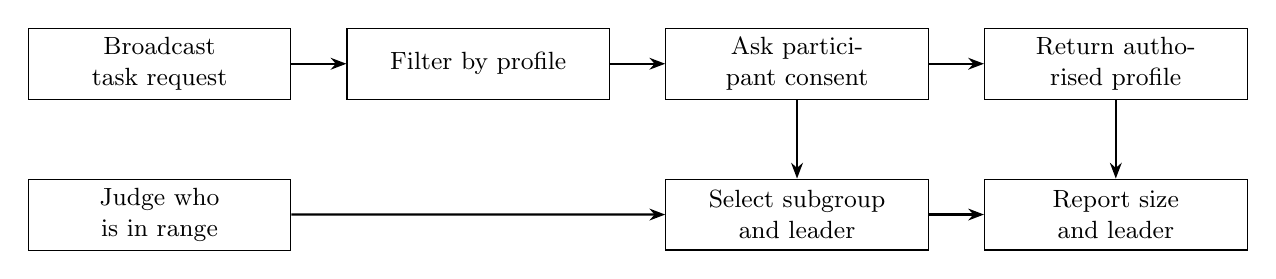
\begin{tikzpicture}[
  box/.style={draw, rectangle, minimum height=9mm, text width=31mm, align=center, font=\small},
  arr/.style={-{Stealth[length=2mm]}, thick}]
\node[box] (b1) {Broadcast task request};
\node[box, right=7mm of b1] (b2) {Filter by profile};
\node[box, right=7mm of b2] (b3) {Ask participant consent};
\node[box, right=7mm of b3] (b4) {Return authorised profile};
\node[box, below=10mm of b1] (c1) {Judge who is in range};
\node[box, below=10mm of b3] (c2) {Select subgroup and leader};
\node[box, below=10mm of b4] (c3) {Report size and leader};
\draw[arr] (b1)--(b2); \draw[arr] (b2)--(b3); \draw[arr] (b3)--(b4);
\draw[arr] (b4)--(c3.north);
\draw[arr] (c1)--(c2);
\draw[arr] (c2)--(c3);
\draw[arr] (b3)--(c2);
\end{tikzpicture}\\[2pt]
{\sm Figure 1. Chosen concept as functions.}
\end{center}

% ---------------------------------------------------------------- 3
\section{Feasibility Case}
Every claim carries its class, its logbook source and a status. Claims C3--C6 are \emph{open} and C2 partly supported because the ESP32 boards are in shipping (L-05).

\begin{center}\footnotesize\setlength{\tabcolsep}{2pt}
\begin{tabular}{@{}p{0.3in}p{0.62in}p{1.5in}p{0.6in}p{0.5in}p{2.1in}p{0.8in}@{}}
\toprule
ID & Tests & Claim & Class & Source & Evidence & Status\\
\midrule
C1 & \req{04} & The watch can run ESP-NOW and BLE advertising together. & Measured & L-04 & Steps 1--8 pass; 31 of 31 send callbacks OK over 30\,s. & Supported\\
C2 & \req{04}, \req{02} & A second device receives the watch's frames, and the reverse. & Measured & L-04 & BLE only: a PC found the advertisement and paired. ESP-NOW, reverse and range untested (Test 1b). & Partly supp.\\
C3 & \req{02} & At least 27 of 30 messages arrive correctly at 30\,m. & Assumed & L-02 & Not tested. Settled by Test 2 (needs beacon). & Open\\
C4 & \req{01}, \req{06} & Watch filtering and consent gate behave correctly. & Measured & L-07 & L-07: Test 6 24/24; Test 7 12/12 (4 accept, 3 reject, 3 timeout, 2 filtered), 4 profile sends, 6 blocked, 0 violations. Abstract skill model on the watch, tap input; radio send and beacon side not tested. & Partly supported\\
C5 & \req{08} & Selection covers all task skills in $\ge 90\,\%$ of trials where a valid subgroup exists. & Measured & L-08 & L-08: hand cases 8/8; 3$\times$1000 simulated trials, 100\,\% covered where a valid subgroup exists (1302 trials), 0 invalid picks, 0 false claims. Abstract skills, no radio; reachability is R1/R2. & Partly supported\\
C6 & R2 & Position from 2D RSSI trilateration agrees with known positions. & Assumed & L-02 & Not tested; needs the three incoming boards (beacon plus two reference points). Tolerance: \pend{value, set before testing}. & Open\\
C7 & \req{07} & The beacon's neighbour record and profile data fit in memory with both stacks active. & Calc.\ + measured & L-03, L-04 & Calc.: at most 26\,B. Measured: 173{,}372\,B heap free after both stacks. Not yet loaded on device. & Partly supp.\\
\bottomrule
\end{tabular}
\end{center}

\subsection*{Evidence for C1 (Test 1a, L-04)}
Watch only (Waveshare ESP32-S3-Touch-AMOLED-2.06, Arduino-ESP32 core 3.3.12, IDF v5.5.5). Wi-Fi station mode and MAC read, ESP-NOW initialisation, callbacks and a broadcast peer, then BLE initialisation, a service and advertising all returned without error (steps 1--7). A 30\,s soak with one broadcast per second plus BLE advertising gave 31 sent, 31 send-callbacks OK, 0 failed.

Internal heap (328{,}324\,B total) fell from 288{,}420\,B at boot to 245{,}980\,B after Wi-Fi ($-42{,}440$), 245{,}824\,B after ESP-NOW ($-156$), 174{,}260\,B after BLE ($-71{,}564$) and 173{,}372\,B at the end of the soak ($-888$); 12{,}564\,B of the 8\,MiB PSRAM was used.

\textbf{What C1 does not show.} A broadcast send-callback only means the frame was transmitted; the watch received nothing from others (rx\,=\,0), as expected with no peer. Step 7 only confirms that the advertising call returned; BLE visibility was checked separately, with a PC (L-04 addendum). That check is not the beacon and not at range. One run, one watch, indoors, USB-powered. Range and delivery are C2 and C3.

\subsection*{Adjacency matrix model (L-03)}
The beacon is node 0 and the $N$ participants are nodes $1$ to $N$, so $n=N+1$. Two nodes are linked if closer than the radio range $R$, and the adjacency matrix has $A_{ij}=1$ if nodes $i$ and $j$ are linked, 0 otherwise. In the instructor's $n=5$ example (order $B,1,2,3,4$; agents 1, 2, 3 hear the beacon, agent 4 hears only agent 3, agents 1--2 and 2--3 hear each other):
\[
\mathbf A=\begin{bmatrix}0&1&1&1&0\\1&0&1&0&0\\1&1&0&1&0\\1&0&1&0&1\\0&0&0&1&0\end{bmatrix}.
\]
The first row is the beacon's row: it says which participants hear the beacon directly, the question the proposal needs answered (R2). Links work both ways, so $\mathbf A=\mathbf A^{\mathsf T}$ and only the upper triangle needs storing, here the bit string $1110\,|\,100\,|\,10\,|\,1$, which cuts $n^2=25$ bits to $n(n-1)/2=10$. The L-03 recommendation is the plain bit matrix for small networks, with the beacon's row kept as its own bit mask. The model assumes a link is either on or off and the same in both directions; that assumption is what C6 tests.

\textbf{Evidence for C7.} For $n=11$ (10 participants plus the beacon) the full matrix is $n^2=121$ bits (16\,B), the upper triangle $n(n-1)/2=55$ bits (7\,B) and the beacon's own row 11 bits. Adding one skill byte per participant (10\,B) gives at most 26\,B, which is 0.015\,\% of the 173{,}372\,B measured free. Storage is not a feasibility risk. A sparse alternative is in Appendix~B (optional).

% ---------------------------------------------------------------- 4
\section{Baselined Requirements}
Baseline is provisional until tests are run. No requirement has been changed.

\begin{center}\sm
\begin{tabularx}{\textwidth}{@{}l l l l Y@{}}
\toprule
ID & Subject & Needs & Status & Reason and next check\\
\midrule
\req{01} & Broadcast requests reach watches & N1, N4, N5 & Open & Keep. Watch-side filtering supported (L-07); delivery needs Test 4.\\
\req{02} & $\ge 90\,\%$ delivery at 30\,m & N4 & Open & Keep. Test 2 (27/30), needs beacon.\\
\req{03} & Two watches at once & N1 & Open & Keep. Test 5, needs second device.\\
\req{04} & Request/response exchange & N1, N2, N4 & Partly supported & Keep. Watch runs both stacks (C1); BLE advertisement found and paired by a PC (C2); exchange with the beacon untested.\\
\req{05} & Removable modules & N4 & Open & Keep. Inspection once beacon is built.\\
\req{06} & Explicit consent before sharing & N2 & Partly supported & Keep. Watch side supported (L-07, 0 violations in 12 runs); full check after beacon.\\
\req{07} & Report group size and leader & N6 & Open & Keep. Test 11; memory sizing supports it (C7).\\
\req{08} & Subgroup covers task skills & N1, N5 & Partly supported & Keep. Selection logic supported in simulation (L-08); reaching the chosen watches needs the boards.\\
\bottomrule
\end{tabularx}
\end{center}

% ---------------------------------------------------------------- 5
\section{Risk Register}
Values below are those of the proposal and are not yet re-estimated; Test 1a does not change any probability. $P=p\times c$, with $p$ and $c$ on 1--4.

\begin{center}\sm
\begin{tabularx}{\textwidth}{@{}l Y c c c c@{}}
\toprule
ID & Risk & $p$ & $c$ & $P$ & Rank\\
\midrule
R1 & Beacon does not deliver messages reliably at 30\,m & 3 & 3 & 9 & 1\\
R2 & Proximity or position not accurate enough for relevant requests & 2 & 3 & 6 & 2\\
R3 & Watch filters requests incorrectly & 2 & 2 & 4 & 3\\
\bottomrule
\end{tabularx}
\end{center}

\begin{center}\sm
\renewcommand{\arraystretch}{1.5}
\begin{tabular}{@{}r|c|c|c|c|@{}}
$p\backslash c$ & 1 & 2 & 3 & 4\\\hline
4 almost certain & \cellcolor{black!10}4 & \cellcolor{black!25}8 & \cellcolor{black!45}\textcolor{white}{12} & \cellcolor{black!65}\textcolor{white}{16}\\\hline
3 likely & \cellcolor{black!10}3 & \cellcolor{black!10}6 & \cellcolor{black!25}\textbf{9 (R1)} & \cellcolor{black!45}\textcolor{white}{12}\\\hline
2 unlikely & 2 & \cellcolor{black!10}\textbf{4 (R3)} & \cellcolor{black!10}\textbf{6 (R2)} & \cellcolor{black!25}8\\\hline
1 rare & 1 & 2 & 3 & \cellcolor{black!10}4\\\hline
\end{tabular}\\[2pt]
{\sm Figure 2. Risk matrix at proposal values; each cell shows $P=p\times c$. Consequence $c$: 1 negligible, 2 moderate, 3 major, 4 severe. Darker cells need attention first.}
\end{center}

\textbf{Top risk, in six fields.}
\begin{center}\sm
\begin{tabularx}{\textwidth}{@{}l Y@{}}
\toprule
Statement & The custom beacon hardware may not deliver messages reliably to a compatible watch at 30\,m (R1).\\
Assumption & The selected wireless interface can deliver beacon messages to the watch at that range under the test conditions.\\
Consequence & Major: \req{02} unmet and every later function depends on the link.\\
Probability & Likely, unchanged. Test 1a shows the watch can run the stacks, not that a frame crosses 30\,m.\\
Evidence required & At least 27 of 30 messages received correctly at a measured 30\,m, unobstructed outdoors (Test 2, C3).\\
Mitigation & Test the link early; if it fails, record the delivery-versus-distance curve (10, 20, 30, 40\,m) and narrow the supported range or change the interface.\\
\bottomrule
\end{tabularx}
\end{center}
\pend{write R2 and R3 in six fields once evidence exists, and re-estimate p}

% ---------------------------------------------------------------- 6
\section{Gate 1 Readiness}
\emph{Draft, to be rewritten after the remaining tests.} The one measured result so far is that the watch runs ESP-NOW and BLE together (C1, L-04) with ample memory (C7). A PC also discovered and paired with the watch's BLE advertisement (C2, partly). Watch-side filtering, consent (C4, L-07) and subgroup selection logic (C5, L-08) are supported in simulation on the watch. No claim about range, delivery or proximity is yet supported (C3, C6); they are open and each names its test. Boards for the beacon and a second node are in shipping (L-05). Provisional expected outcome: \textbf{proceed with conditions}, the condition being the 30\,m delivery test once the boards arrive. \pend{confirm outcome and arrival date}

% ================================================================ appendices
\clearpage
\appendix
\section{Logbook Extracts}
\begin{center}\sm
\begin{tabularx}{\textwidth}{@{}l l Y@{}}
\toprule
Entry & Date & Content\\
\midrule
L-02 & 2026-10-23, 2026-11-06 & Research on links (ESP-NOW, Bluetooth LE, external transceiver) and positioning (trilateration, triangulation); entry below.\\
L-03 & 2026-11-13 & Session with instructor on storing connectivity between wireless agents and a beacon. The adjacency matrix is the relevant part (Section~3); sparse (CSR) storage is optional background (Appendix~B). The HTML/JS simulator \texttt{beacon\_app.html} is to be extended with the RSSI data gathered in testing. Files: \texttt{beacon\_storage.tex/pdf}, \texttt{beacon\_sim.py}, \texttt{beacon\_app.html}, \texttt{beacon\_network.png}.\\
L-04 & 2026-11-13 & Test 1a, below.\\
L-05 & 2026-11-13 & Three ESP32 boards in shipping: the beacon and two further reference points, which give the three reference points 2D trilateration needs (L-02). Expected arrival \pend{date}. Tests 1b and 2--5 and the RSSI measurements are open until they arrive.\\
L-06 & 2026-11-13 & Criteria and weights for Section~2 (coverage 0.35, uncertainty 0.25, buildability 0.25, cost 0.15), written before scoring; chosen by the assistant at the author's request, \pend{author confirms}.\\
L-07 & 2026-11-13 & Tests 6 and 7 on the watch screen: 24/24 and 12/12, overall PASS, touch input.\\
L-08 & 2026-11-13 & Test 10, subgroup selection on the watch: hand cases 8/8, 3$\times$1000 random trials, overall PASS.\\
\bottomrule
\end{tabularx}
\end{center}
L-01 (early brainstorming) predates the proposal and is not reproduced here.

\subsection*{L-02, 2026-10-23 and 2026-11-06, assumed: link and positioning research}
\textbf{Objective.} Compare candidate links and positioning methods for R1 and R2. \textbf{Class.} Secondary sources only, nothing measured, so every figure is \emph{assumed}. Only the ESP-NOW description cites a source (Espressif, \texttt{espressif.com/en/solutions/low-power-solutions/esp-now}); \pend{sources for the range figures}.

\begin{center}\footnotesize\setlength{\tabcolsep}{4pt}
\begin{tabular}{@{}l l l p{2.6in}@{}}
\toprule
Link & Clear / outdoors & Obstacles / indoors & Notes\\
\midrule
Wi-Fi 2.4\,GHz (ESP32-S3) & 35--50\,m & 15--20\,m & ESP-NOW runs on this radio\\
Bluetooth 5.0 & 30--40\,m & 10--15\,m & standard mode\\
BLE Long Range (Coded PHY) & 100--200+\,m & 20--40\,m & \\
nRF24L01 (2.4\,GHz) & 30--100\,m & 10--30\,m & hurt by walls, concrete floors, 2.4\,GHz traffic; external antenna: 700--1000\,m outdoors, 30--100+\,m indoors; external modules needed\\
\bottomrule
\end{tabular}
\end{center}

\textbf{Positioning notes.} Trilateration: distances from three or more reference points; in 2D three circles give one position (one point gives a circle, two give two intersections). In 3D three points leave two positions and four are used in the real world, the fourth correcting a clock error as in GPS, which is not needed here. Triangulation: two or more angular lines of sight; in 2D a baseline between two points and two measured angles; needs direct line of sight. RSSI: reference points 5--10\,m apart, works with any ESP32 module, precision not required. Wi-Fi FTM/RTT: ESP32-S and -C series only. \textbf{To look into:} multipath interference and signal attenuation (indoor transmission).

\textbf{Reasons recorded} (author to confirm wording).
\begin{itemize}\setlength\itemsep{0pt}
\item ESP-NOW stays a candidate: built into the watch's chip, fast and low power, suits one beacon controlling many watches, and the beacon only needs an ESP-family board.
\item External transceiver not preferred: needs external modules at both ends (cost), the watch has only Wi-Fi and BLE (proposal), and indoor range is hurt by walls and 2.4\,GHz traffic.
\item Triangulation set aside: needs angle measurements and direct line of sight, while RSSI from received packets gives strength, not direction.
\item Wi-Fi FTM/RTT set aside: only on ESP32-S and -C series; RSSI works on any ESP32 module and the application does not need precise ranging.
\item Undecided: ESP-NOW or BLE as the link; the author leans to BLE Long Range for its 20--40\,m through obstacles but is not sure.
\end{itemize}

\subsection*{L-04, 2026-11-13, measured: Test 1a, can the watch run the candidate links?}
{\sloppy\textbf{Objective.} Check that ESP-NOW and BLE initialise and run together on the watch (supports \req{04}, R1). \textbf{Device.} Waveshare ESP32-S3-Touch-AMOLED-2.06, Arduino IDE, Arduino-ESP32 core 3.3.12, IDF v5.5.5, chip ESP32-S3 rev 2, 240\,MHz, flash 33{,}554{,}432\,B (32\,MiB), PSRAM 8\,MiB. \textbf{Code.} \texttt{code/test1a\_watch\_link\_check.ino}. \textbf{Pass criterion} (stated in the sketch header before the run): steps 1--7 pass and no send failures in a 30\,s soak. \textbf{Environment and power:} indoors, USB-powered; antenna orientation not recorded. \textbf{N:} one run, 31 broadcasts. \textbf{Result:} OVERALL PASS; tx OK 31, tx fail 0, received from others 0.}

\textbf{Anomalies and limits.} Step 7 reports pass unconditionally after the advertising call, so it alone does not show BLE visibility. ESP-NOW callback success is not proof of reception. The sketch's setup note said 16\,MB flash; the board reports 32\,MiB, which does not affect the result.

\textbf{Addendum, 2026-11-13, measured (BLE only).} Using Microsoft Bluetooth LE Explorer on a PC, the author found the watch's advertisement (name \texttt{T1a-watch}) and paired with it. Not recorded: \pend{PC model and OS, distance, how many attempts}. This shows another device can discover and pair over BLE; it does not show message delivery, range, ESP-NOW reception, or reception by the beacon.

\textbf{Raw serial output} (\texttt{logs/L-04\_test1a\_serial.txt}):
{\footnotesize\verbatiminput{logs/L-04_test1a_serial.txt}}

\subsection*{L-07, 2026-11-13, planned: Tests 6 and 7, filtering and consent gate on the watch}
\textbf{Objective.} Check that the watch filters requests correctly (\req{01}, R3) and shares profile data only after the participant accepts on the watch (\req{06}). \textbf{Code.} \texttt{code/test6\_7\_filter\_consent.ino}. \textbf{Model.} Eight abstract skills A--H as a bitmask; a request is relevant if the participant is available and shares at least one skill. \textbf{Test 6.} 24 hand-written cases (skill rule alone, availability alone, combined); pass: 24 of 24. \textbf{Test 7.} 12 runs (4 accept, 3 reject, 3 timeout, 2 non-matching) on the watch screen; pass: every run as expected, profile sent exactly once in each accept run and never otherwise, zero violations. \textbf{Limits.} The tap stands in for the final interface and the TX line for the radio send, so \req{06} is supported on the watch side only. \textbf{Input mode:} touch screen (touch controller found at 0x38). \textbf{Result, same day:} Test 6, 24 of 24 correct. Test 7, 12 of 12 runs as expected: runs 1--4 accepted, 5--7 rejected, 8--10 timed out, 11--12 filtered; profile sent 4 times (accept runs only), 6 requests blocked by the gate, 0 violations. Overall PASS, first attempt. Serial log: \texttt{logs/L-07\_test6\_7\_serial.txt}. The sketch first failed to compile (enum types used before definition by the IDE's auto-prototypes) and was fixed before this run. \textbf{Limits.} Abstract skills, tap in place of the final interface, TX line in place of the radio; the 12 runs are scripted, so this shows the logic is correct, not that people respond reliably.

\subsection*{L-08, 2026-11-13: Test 10, subgroup selection covers the task skills}
\textbf{Objective.} Check that a selection rule picks a subgroup covering every required skill whenever one exists, and says so honestly when none does (\req{08}, C5). \textbf{Code.} \texttt{code/test10\_selection.ino}. \textbf{Model.} Eight abstract skills A--H as a bitmask; rule under test: greedy cover (repeatedly pick the available participant adding the most missing required skills). A candidate rule, not fixed by the proposal. \textbf{Part A.} 8 hand-worked cases; pass 8 of 8. \textbf{Part B.} 3 batches of 1000 random trials (seeds 1--3; rosters of 2--10; each skill held with probability 1/4; 80\,\% available; task needs 2--4 skills), checked by two independent methods (coverage test, brute-force minimum subgroup). Pass, in every batch: $\ge 90\,\%$ of feasible trials covered, 0 invalid picks, 0 false ``covered'' claims, at least 100 feasible and 1 infeasible trial; subgroup size reported only. \textbf{Result.} Part A 8/8. Feasible trials 440, 418, 444 (infeasible 560, 582, 556): 100.0\,\% covered in each, 0 invalid picks, 0 false claims. Mean size greedy 1.83 against minimum 1.82; equal to the minimum in 99.4\,\% of covered trials, worst excess one participant (hand case 3 shows a non-minimal pick on purpose). Overall PASS, first run; run time 127\,ms. The watch's figures matched my host check exactly, as expected from fixed seeds. Result summary: \texttt{logs/L-08\_test10\_summary.txt}. \textbf{Limits.} This rule covers the task whenever a valid subgroup exists, so the 90\,\% threshold is met by construction; the informative results are the zero false claims and the size. Abstract skills, simulated rosters, no radio: reaching the chosen participants is R1 and R2.

\textbf{AI use.} Test code and this document's scaffolding were produced with an AI assistant from the instructor's guide, the proposal and the instructor session; results are the author's measurements and must be checked against the logbook.

\clearpage
\section{Optional: Sparse (CSR) Storage and Illustrative Network (from L-03)}
\textbf{Not needed by the proposal.} The instructor marked the adjacency matrix (Section~3) as the relevant part; the sparse form below is background that is nice to have.

When each node hears only a few others, store only each node's neighbours. For the $n=5$ example the adjacency list is $0\!:\!1,2,3;\ 1\!:\!0,2;\ 2\!:\!0,1,3;\ 3\!:\!0,2,4;\ 4\!:\!3$, kept in memory as two flat arrays (compressed sparse row, CSR): the joined neighbour lists, and where each node's list starts,
\[
\text{neighbours}=[1,2,3,\,0,2,\,0,1,3,\,0,2,4,\,3],\qquad \text{start}=[0,3,5,8,11,12].
\]
With $E$ links, each stored twice, and each number written with $\lceil\log_2 n\rceil$ bits, the list costs
\[
S_{\text{list}}=2E\lceil\log_2 n\rceil\ \text{bits}=2\cdot 6\cdot 3=36\ \text{bits}\quad(n=5,\ E=6),
\]
more than the 25-bit matrix. The list wins only when the mean degree $\bar k<n/\lceil\log_2 n\rceil$. For $n=11$, $\lceil\log_2 11\rceil=4$, so $S_{\text{list}}=8E$ bits against 121 bits (full) or 55 bits (triangle): the list wins only for $\bar k<2.75$ against the full matrix, or $E\le 6$ links against the triangle. The plain matrix is the right choice here.

\begin{center}
\includegraphics[width=0.9\textwidth]{figures/fig_connectivity_bw.png}\\[2pt]
{\sm Figure 3. Illustrative network, $N=18$, $R=1$ (beacon\,=\,star; circles, squares, triangles\,=\,1, 2, 3 hops). Seed 12 was found by searching seeds for a beacon degree of 6 and a maximum of 3 hops, so this is an \emph{example}, not evidence about how often such networks occur. Redrawn in greyscale from \texttt{beacon\_sim.py}.}
\end{center}

\textbf{Limits of the model.} (i) Links are treated as on or off and the same both ways; real radio links need not be, which is why C6 is open until measured. (ii) The project has 10 participants, not 18. (iii) Agent-to-agent links and hop counts appear only in the example and figure; they are outside the proposal's scope.

\end{document}